\problemname{Congklak}

\illustration{0.3}{illustration.png}{
   A typical Congklak game board. \\
   CC BY-SA 4.0 by rikadiani17 on \href{https://pixabay.com/illustrations/congklak-game-game-play-5943996/}{Pixabay}
}%
%
Alice and Bill really enjoy playing board games, and they are always looking for new challenges.
Recently, they discovered the Indonesian game \textit{Congklak} which is played with a game board made up of several holes containing some number of stones.
After playing some games, Alice quickly got the hang of it and won every game, so Bill did not want to play any more.
Instead, inspired by the rules of the game, he came up with the following challenge for Alice:

There is a game board with $n$ holes arranged in a long row.
These holes are numbered from $1$ to $n$ from left to right.
Initially the $i$th hole contains $a_i$ stones.
Note that this setup differs from the usual Congklak game,
where the game board consists of two rows and one large hole at each end.

Now Bill will play $t$ games where each game goes as follows:

Bill starts the game at the first hole, holding one new stone in his hand.
He then moves along the game board from hole $1$ to hole $n$.
At each hole $i$, he first checks how many stones are currently in the hole,
and depending on the result he performs exactly one of the following two actions:
\begin{itemize}
    \item[i)]
        If the hole is empty, he drops one stone into it.
        Next, he checks how many stones are still in his hand.
        If his hand is empty, the game stops.
        Otherwise, he moves his hand to hole $i+1$ next and repeats the steps.
    \item[ii)]
        If there is at least one stone in the hole, he also drops one stone into it.
        Next, he checks how many stones are still in his hand.
        If his hand is empty, he takes out all the stones from hole $i$ into his hand.
        Regardless of whether or not his hand was empty, he moves his hand to hole $i+1$ next and repeats the steps.
\end{itemize}
When Bill moves his hand past hole $n$, the game stops and Bill discards any stones that he still holds in his hand.

Bill challenges Alice to predict in advance the number of stones in every hole after playing exactly $t$ games.
Note that the game board is \textbf{not} reset after playing a game,
i.e.\ the initial configuration of the second game is the same as the configuration when the first game ends.

\begin{Input}
The input consists of:
\begin{itemize}
  \item One line with two integers $n$ and $t$ ($1 \leq n \leq 10^5$, $1 \leq t \leq 10^{12}$),
  the number of holes and the number of games.
  \item One line with $n$ integers $a_1, \ldots, a_n$ ($0 \leq a_i \leq 10^{12}$),
  where $a_i$ describes the initial number of stones in the $i$th hole.
\end{itemize}
\end{Input}

\begin{Output}
Output $n$ integers, the $i$th of which is the number of stones in hole $i$ after playing $t$ games.
\end{Output}

\section*{Notes}
In the first sample, Bill plays exactly one game. The figure below visualizes the steps performed during this game.

In the second sample, the initial number of stones per hole is $[1000000000000, 1, 2, 3]$.
The number of stones per hole after each game is:
\begin{enumerate}
  \item $[0, 2, 3, 4]$
  \item $[1, 2, 3, 4]$
  \item $[0, 3, 0, 5]$
  \item $[1, 3, 0, 5]$
\end{enumerate}

\vspace{5ex}

\begin{figure}[h]
  \centering
  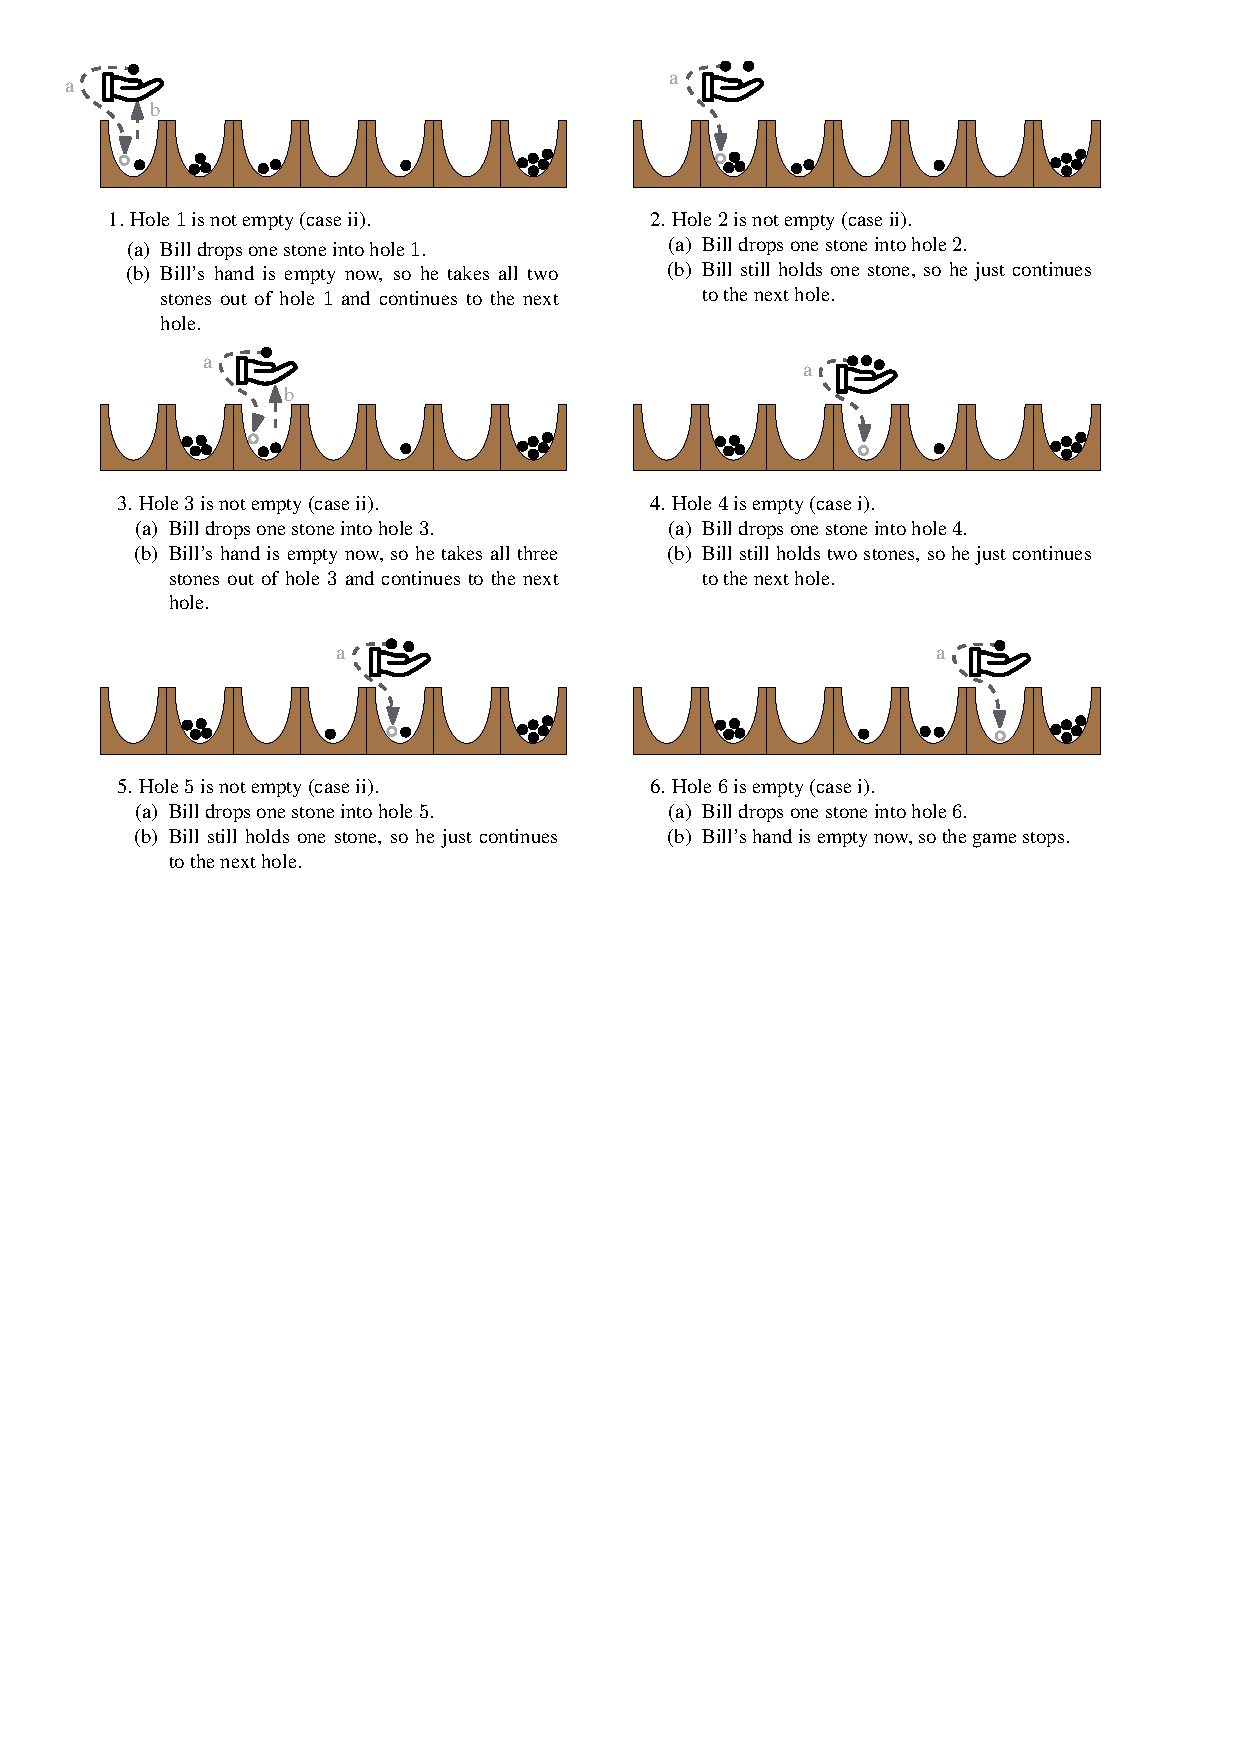
\includegraphics[width=\textwidth]{sample-vis.pdf}
  \caption{Visualization of the only game which Bill plays in the first sample. \\
  {\scriptsize Hand icon: MIT Licence by jtblabs on \href{https://www.svgrepo.com/svg/473219/hand-holding/}{svgrepo}}}
\end{figure}
